% ============================================================================
% Section 6: Ablation Studies
% ============================================================================
\section{Ablation Studies}
\label{sec:ablation-study}

We report five completed ablation analyses
grouped into four run families: embedding text; dense, hybrid, and graph
retrieval as one joint retrieval/graph family; reranking; and generator
prompting. Comparisons are made within a family because candidate
construction, context budgets, output limits, and latency accounting differ;
the results are not treated as one pooled factorial experiment.

\subsection{Embedding Text Ablation: Chunk-Only versus Chunk+Metadata}
\label{sec:ablation-chunk-meta}

This comparison holds the dense encoder, generator, benchmark, seed, and raw
FAISS evaluation path fixed. Only the indexed text changes from the chunk body
to a header-plus-chunk representation. On 400 paired answerable questions,
exact chunk Recall@10 is effectively unchanged: both variants round to
48.5\%, with an unrounded metadata-minus-chunk-only difference of only
+0.08 percentage points (reported as +0.1 pp in
\hyperref[tab:embedding-results]{Table~\ref*{tab:embedding-results}}).
Metadata nevertheless increases document-level success at rank 10 from
65.8\% to 70.2\%, a paired gain of +4.5 pp (95\% CI [+0.5,+8.8]), while
MRR@10 decreases by 5.9 pp (95\% CI [$-9.1,-2.7$]).

Because the metadata representation includes both document titles and
provision headers, we additionally report provision-level success. At rank
10, provision success is 53.8\% for chunk-only retrieval and 53.5\% for
chunk+metadata, a negligible $-0.25$ pp difference (95\% CI
[$-5.0,+4.5$]). At rank 5, provision success decreases from 44.3\% to
40.3\%. Thus, the observed metadata gain is concentrated at document
discovery rather than provision identification or exact chunk ranking. The
retrieval curves and paired outcomes are shown in
\hyperref[fig:embedding-ablation]{Figure~\ref*{fig:embedding-ablation}}.

\begin{figure*}[t]
\centering
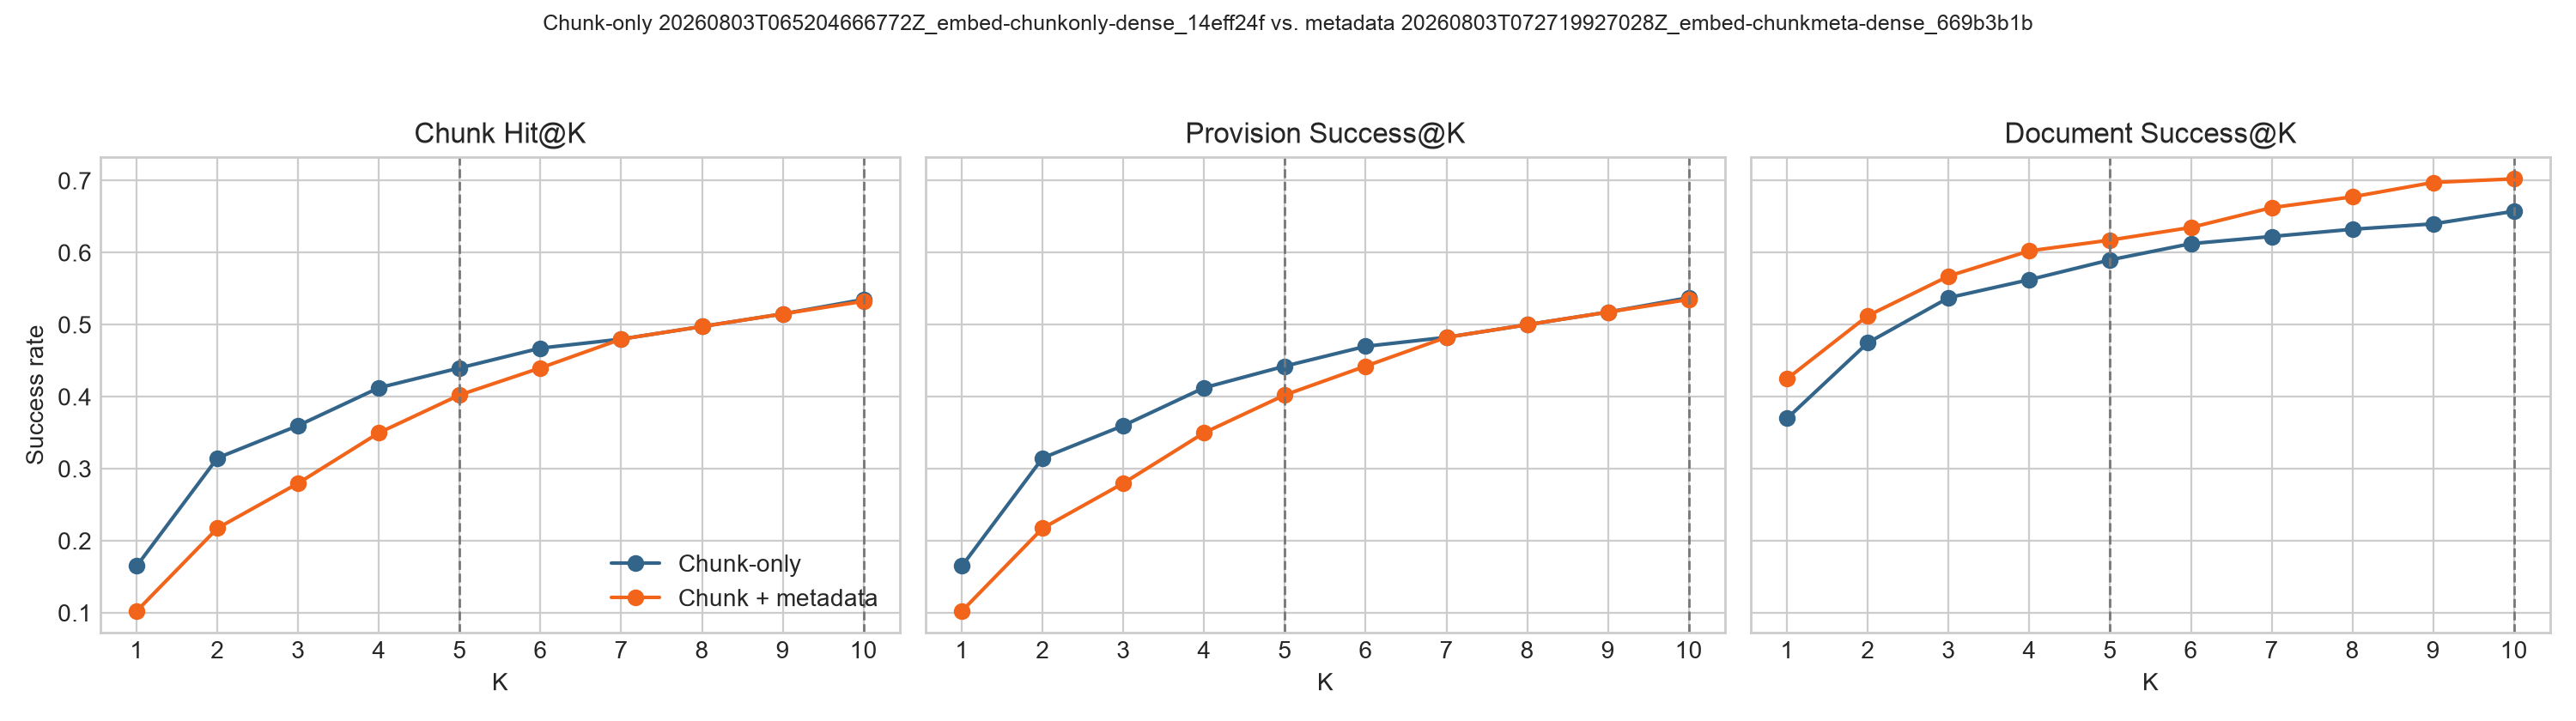
\includegraphics[width=0.48\textwidth]{../../ablation_study/chunkOnly_vs_chunkMetadata/results/success_at_k_curve.png}
\hfill
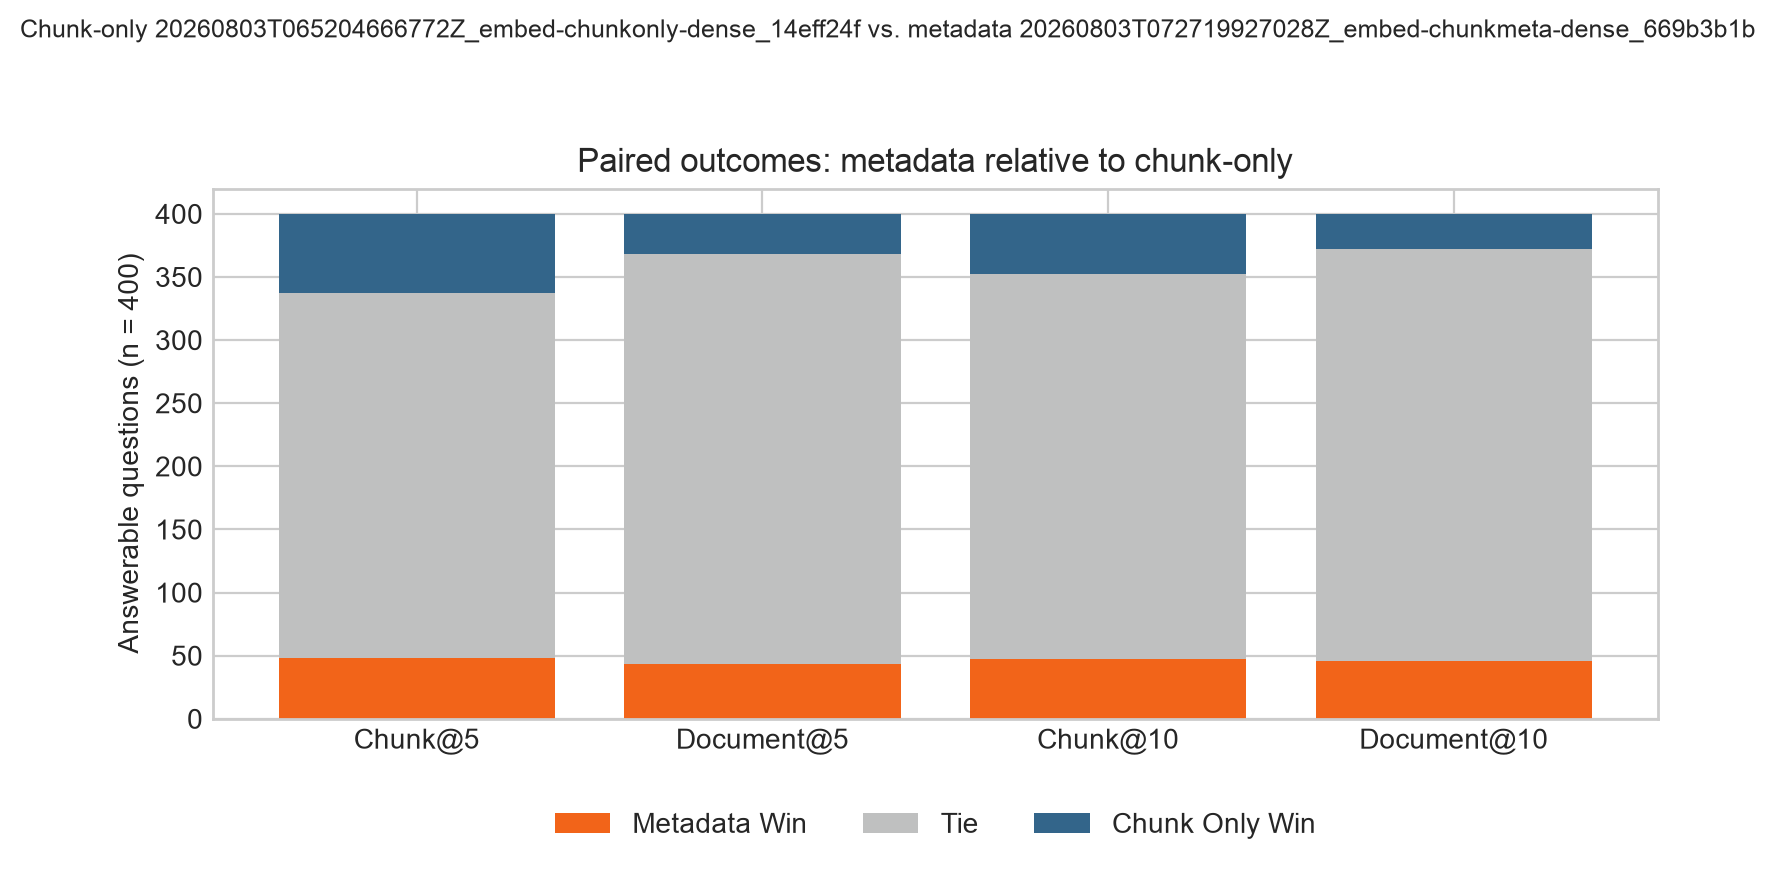
\includegraphics[width=0.48\textwidth]{../../ablation_study/chunkOnly_vs_chunkMetadata/results/paired_win_tie_loss.png}
\caption{Embedding-text ablation diagnostics. The left panel shows success
curves by retrieval depth; the right panel shows paired win, tie, and loss
counts. Both plots use the shared answerable-question comparison.}
\label{fig:embedding-ablation}
\end{figure*}

\begin{table*}[t]
\centering
\scriptsize
\caption{Embedding-text ablation on 400 paired answerable questions. Values
are percentages. Document and provision success denote retrieval of at least one
chunk from a gold document or gold provision, respectively. Deltas are
chunk+metadata minus chunk-only. Recall@10 values in the two rows both round
to 48.5\%; the unrounded difference is +0.08 pp.}
\label{tab:embedding-results}
\resizebox{\textwidth}{!}{%
\begin{tabular}{lrrrrrrrrrr}
\toprule
\textbf{Variant} & \textbf{Hit@5} & \textbf{Recall@5} & \textbf{MRR@5} &
\textbf{Doc@5} & \textbf{Prov@5} & \textbf{Hit@10} &
\textbf{Recall@10} & \textbf{MRR@10} & \textbf{Doc@10} &
\textbf{Prov@10} \\
\midrule
Chunk-only & 44.0 & 39.0 & 27.4 & 59.0 & 44.3 & 53.5 & 48.5 & 28.6 & 65.8 & 53.8 \\
Chunk+metadata & 40.2 & 36.8 & 20.9 & 61.8 & 40.3 & 53.2 & 48.5 & 22.7 & 70.2 & 53.5 \\
Delta & $-3.8$ & $-2.2$ & $-6.5$ & $+2.8$ & $-4.0$ & $-0.2$ &
$+0.1$ & $-5.9$ & $+4.5$ & $-0.3$ \\
\bottomrule
\end{tabular}%
}
\end{table*}
\subsection{Retrieval Ablation: Dense versus Hybrid Retrieval}
\label{sec:ablation-retrieval}

The dense/hybrid comparison uses the same header-plus-chunk dense index,
50-seed retrieval budget, 10-chunk final context, benchmark, and generator.
Hybrid retrieval adds ten sharded BM25 indexes and reciprocal rank fusion.
DenseOnly outperforms
HybridOnly on Recall@10 (48.55\% versus 42.57\%) and nDCG@10 (0.2813 versus
0.2638); the full comparison is in
\hyperref[tab:dense-hybrid-results]{Table~\ref*{tab:dense-hybrid-results}}.
The paired Recall@10 difference is $-5.98$ points with a 95\% CI of
[$-9.71,-2.21$]. Hybrid retrieval also raises recorded total median latency
from 5.483 seconds to 31.538 seconds. The hybrid total includes 26.990 seconds
per query amortized from 13,495 seconds of BM25 batch precomputation over the
500-question batch; this accounting is distinct from online request latency.
Paired uncertainty is reported in
\hyperref[tab:dense-hybrid-paired]{Table~\ref*{tab:dense-hybrid-paired}}.

\begin{table*}[t]
\centering
\scriptsize
\caption{Dense versus hybrid retrieval. Retrieval values use 400 answerable
questions; latency percentiles use all 500 cases. The fallback column is the
fraction of 100 unanswerable outputs containing the family-specific Vietnamese
fallback phrase.}
\label{tab:dense-hybrid-results}
\resizebox{\textwidth}{!}{%
\begin{tabular}{lrrrrrrr}
\toprule
\textbf{Method} & \textbf{Recall@5} & \textbf{Recall@10} &
\textbf{MRR@10} & \textbf{nDCG@10} & \textbf{Retrieval p50/p95} &
\textbf{Total p50/p95} & \textbf{Fallback} \\
\midrule
DenseOnly & 0.3678 & 0.4855 & 0.2267 & 0.2813 & 0.797/0.856 & 5.483/9.946 & 0.38 \\
HybridOnly & 0.3140 & 0.4257 & 0.2252 & 0.2638 & 27.855/27.924 & 31.538/33.623 & 0.38 \\
\bottomrule
\end{tabular}%
}
\end{table*}

\begin{table}[t]
\centering
\scriptsize
\caption{Paired hybrid-minus-dense differences.}
\label{tab:dense-hybrid-paired}
\begin{tabular}{lrr}
\toprule
\textbf{Metric} & \textbf{Mean delta} & \textbf{95\% CI} \\
\midrule
Recall@10 & $-0.0598$ & $[-0.0971,-0.0221]$ \\
MRR@10 & $-0.0015$ & $[-0.0299,+0.0271]$ \\
nDCG@10 & $-0.0175$ & $[-0.0437,+0.0085]$ \\
\bottomrule
\end{tabular}
\end{table}

\subsection{Graph Ablation: With versus Without Graph Expansion}
\label{sec:ablation-graph}

Graph variants expand the top five seed chunks within their parent provisions
with \texttt{max\_hop=1}, replace the baseline top-10 context, and retain at
most 10 chunks. They use broad validity filtering without a query-time
validity overlay or reranking, so this comparison evaluates the complete
context-selection policy rather than graph traversal in isolation. Graph
expansion currently displaces more evidence than it adds.
Relative to DenseOnly, DenseGraph changes Recall@10 by $-12.40$ points and
loses at least one previously retrieved gold chunk for 61 questions while
adding a graph-only gold chunk for only one question. The HybridOnly to
HybridGraph change is $-11.81$ points, with 59 questions losing a gold chunk
and six gaining one; the displacement counts and rank deltas are summarized in
\hyperref[tab:graph-effect]{Table~\ref*{tab:graph-effect}}.

Graph contexts are denser because they contain fewer chunks on average (5.605
for DenseGraph and 6.305 for HybridGraph), and their identity precision is
higher. This is a precision--coverage trade-off, not evidence of an overall
retrieval-quality improvement. Of the 65 gold-chunk occurrences lost by
DenseGraph, 60 were outside the original top-five seeds; for HybridGraph, 52
of 60 were outside the original top five. The counts support seed-preserving
expansion as the next controlled graph test.

\begin{table*}[t]
\centering
\scriptsize
\caption{Effect of graph expansion on top-10 gold evidence. Counts are over
400 answerable questions; graph-only gold is introduced by expansion and
graph-missed gold was present before expansion but absent afterward. The
fallback column is the fraction of 100 unanswerable outputs containing the
family-specific Vietnamese fallback phrase.}
\label{tab:graph-effect}
\resizebox{\textwidth}{!}{%
\begin{tabular}{lrrrrrrrr}
\toprule
\textbf{Base} & \textbf{$\Delta$ Recall@10} & \textbf{$\Delta$ MRR@10} &
\textbf{$\Delta$ nDCG@10} & \textbf{Graph-only gold} &
\textbf{Graph-missed gold} & \textbf{Avg. chunks} & \textbf{ID precision} &
\textbf{Fallback} \\
\midrule
DenseOnly $\rightarrow$ DenseGraph & $-0.1240$ & $-0.0222$ & $-0.0439$ &
1 query (0.25\%) & 61 queries (15.25\%) & 5.605 & 0.0800 & 0.41 \\
HybridOnly $\rightarrow$ HybridGraph & $-0.1181$ & $-0.0240$ & $-0.0411$ &
6 queries (1.50\%) & 59 queries (14.75\%) & 6.305 & 0.0641 & 0.47 \\
\bottomrule
\end{tabular}%
}
\end{table*}

\subsection{Reranker Ablation}
\label{sec:ablation-reranking}

The reranker family compares no reranking, RRF-only, mMiniLM, Qwen3, BGE,
and Jina over a reconstructed shared RRF pool of 30 candidates and a final
top 10. All six runs cover the same 500 questions without retrieval or
generation errors, and the reconstruction matches the recorded RRF-only
top-10 prefix for 500/500 questions. Candidate Recall@30 is 0.5995 and
Candidate Hit@30 is 0.6450 for every configuration, so the comparison measures
ranking and retention within a fixed evidence ceiling.

Jina is the strongest retrieval configuration: relative to RRF-only, it
improves Recall@10 by +9.23 points, MRR@10 by +13.35 points, and nDCG@10 by
+11.85 points; all three 95\% paired-bootstrap intervals exclude zero. Qwen3
and BGE also have positive intervals, while mMiniLM supplies a smaller
positive gain at the lowest reranker cost. BGE has the highest token F1 and
ROUGE-L, whereas Jina has the highest observed unanswerable accuracy. These
answer metrics are lexical and abstention diagnostics, not legal correctness
judgments. Aggregate scores and latency are linked in
\hyperref[tab:reranker-results]{Table~\ref*{tab:reranker-results}}, with
paired effects in \hyperref[tab:reranker-paired]{Table~\ref*{tab:reranker-paired}}
and diagnostic curves in \hyperref[fig:reranker-curves]{Figure~\ref*{fig:reranker-curves}}.

\begin{table*}[t]
\centering
\scriptsize
\caption{Multi-reranker ablation over a shared 30-candidate pool and final
top-10 context. Retrieval and overlap values are means over 400 answerable
questions; recorded unanswerable accuracy and p50 latency use the complete
500-case runs.}
\label{tab:reranker-results}
\resizebox{\textwidth}{!}{%
\begin{tabular}{lrrrrrrrrr}
\toprule
\textbf{Model} & \textbf{Recall@10} & \textbf{Hit@10} & \textbf{MRR@10} &
\textbf{nDCG@10} & \textbf{Token F1} & \textbf{ROUGE-L} &
\textbf{Unans. acc.} & \textbf{Rerank p50} & \textbf{Total p50} \\
\midrule
None & 0.4842 & 0.5375 & 0.2167 & 0.2714 & 0.2801 & 0.2453 & 0.856 & 0.000 & 2.925 \\
RRF-only & 0.4382 & 0.4800 & 0.2335 & 0.2728 & 0.2750 & 0.2416 & 0.874 & 0.000 & 2.972 \\
mMiniLM & 0.4973 & 0.5425 & 0.3047 & 0.3425 & 0.2901 & 0.2568 & 0.872 & 0.385 & 3.343 \\
Qwen3 & 0.5218 & 0.5725 & 0.3418 & 0.3688 & 0.2912 & 0.2583 & 0.876 & 9.695 & 13.007 \\
BGE & 0.5188 & 0.5675 & 0.3247 & 0.3593 & \textbf{0.2955} & \textbf{0.2603} & 0.868 & 2.872 & 5.848 \\
Jina & \textbf{0.5305} & \textbf{0.5850} & \textbf{0.3670} &
\textbf{0.3914} & 0.2913 & 0.2558 & \textbf{0.884} & 1.278 & \textbf{4.158} \\
\bottomrule
\end{tabular}%
}
\end{table*}

\begin{table*}[t]
\centering
\scriptsize
\caption{Paired effects of each reranker relative to RRF-only. Deltas are in
percentage points; intervals are 95\% percentile bootstrap CIs from 10,000
question-level resamples over the 400 answerable cases. A negative false
refusal delta indicates fewer refusals on answerable questions.}
\label{tab:reranker-paired}
\resizebox{\textwidth}{!}{%
\begin{tabular}{lrrrr}
\toprule
\textbf{Reranker} & \textbf{$\Delta$ Recall@10} & \textbf{$\Delta$ MRR@10} &
\textbf{$\Delta$ nDCG@10} & \textbf{$\Delta$ false refusal} \\
\midrule
mMiniLM & $+5.91$ [$+1.85,+9.96$] & $+7.12$ [$+3.55,+10.68$] &
$+6.96$ [$+3.77,+10.26$] & $+0.25$ [$-3.00,+3.50$] \\
Qwen3 & $+8.37$ [$+4.57,+12.25$] & $+10.84$ [$+7.24,+14.36$] &
$+9.60$ [$+6.52,+12.73$] & $-0.25$ [$-3.25,+2.75$] \\
BGE & $+8.07$ [$+4.29,+11.80$] & $+9.12$ [$+5.50,+12.70$] &
$+8.65$ [$+5.47,+11.84$] & $+0.75$ [$-2.25,+3.75$] \\
Jina & $+9.23$ [$+5.51,+12.98$] & $+13.35$ [$+9.51,+17.24$] &
$+11.85$ [$+8.46,+15.27$] & $-1.25$ [$-4.00,+1.25$] \\
\bottomrule
\end{tabular}%
}
\end{table*}

\begin{figure*}[t]
\centering
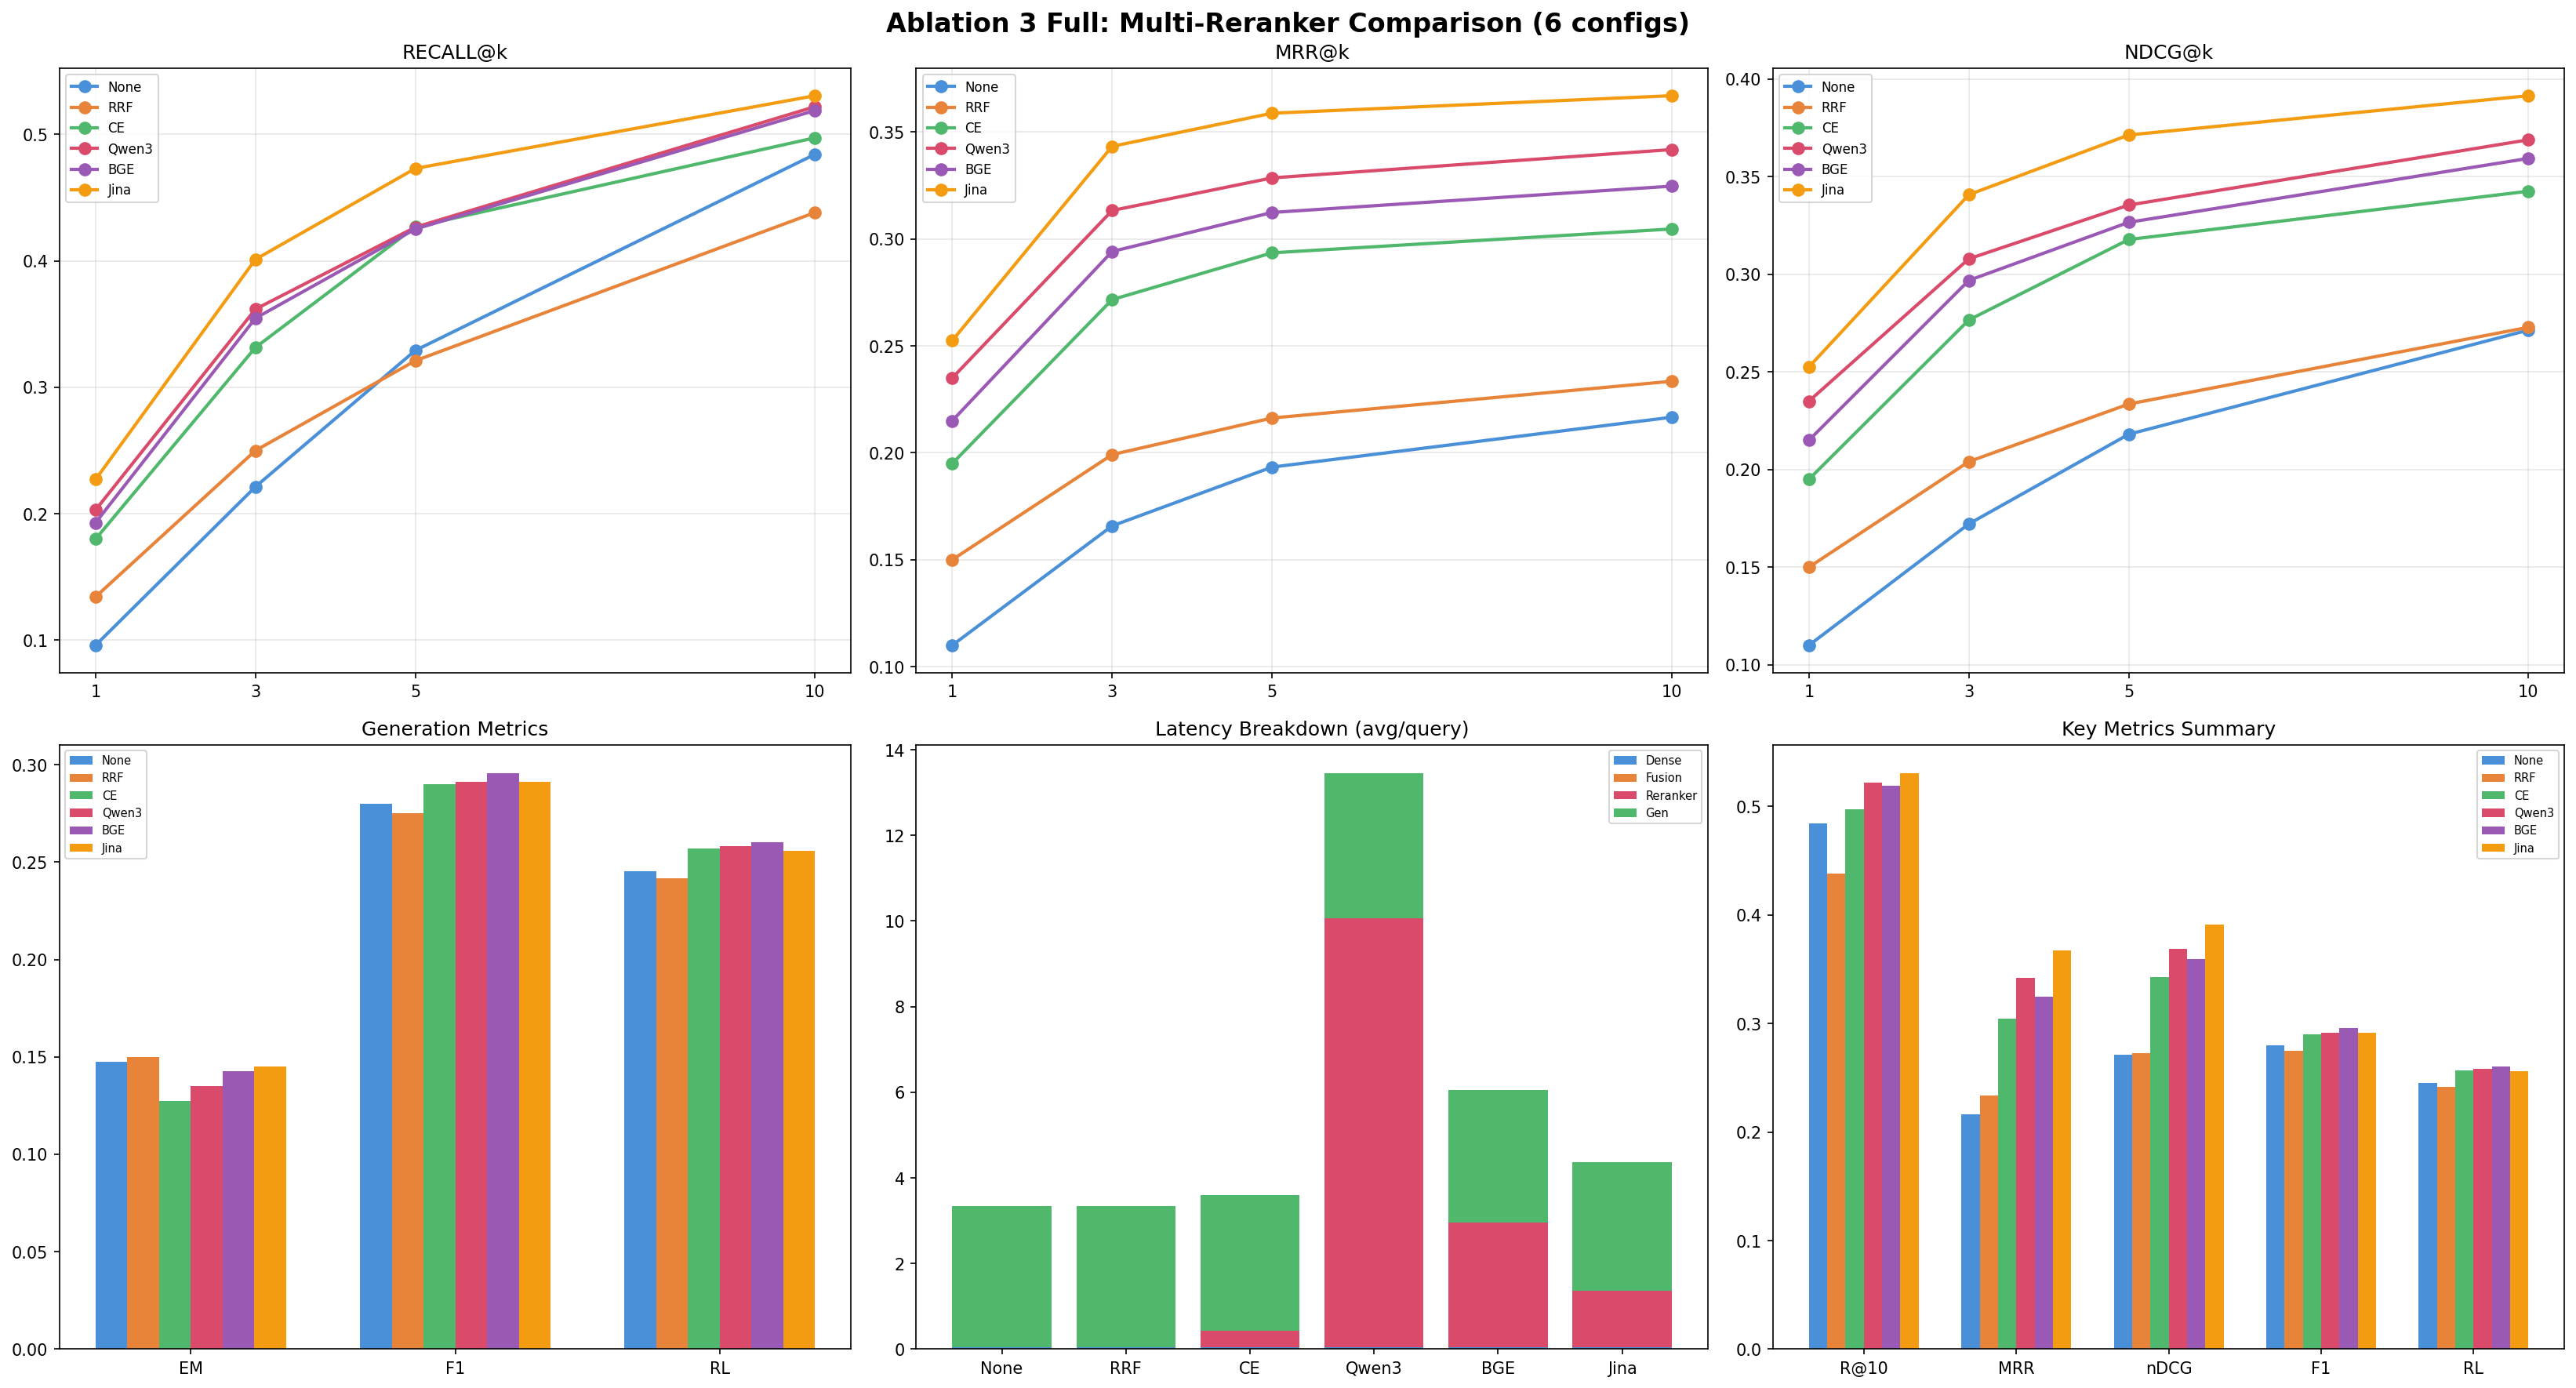
\includegraphics[width=\textwidth]{../../ablation_work/reranker_choices/evaluation_runs/ablation3_reranker_v2/charts.png}
\caption{Reranker curves, answer-overlap diagnostics, latency breakdown, and
headline metrics from the six-configuration run. The paired confidence
intervals in Table~\ref{tab:reranker-paired} are the primary uncertainty
analysis.}
\label{fig:reranker-curves}
\end{figure*}

\subsection{Generator Ablation: Base Prompt versus Chain-of-Thought Prompt}
\label{sec:ablation-reasoning}

The generator-reasoning family keeps the intended retrieved top-10 context
fixed for each question and changes the prompt mode. The primary comparison
uses complete GPT-4o-mini Base and CoT runs: both cover all 500 benchmark
questions and share 400 answerable question IDs. The frozen artifacts report
zero retrieval-context mismatches. The DeepSeek-V3.1-Thinking, GLM-5, and
Qwen3-8B pairs are complete but descriptive; four shared DeepSeek cases have
different exact top-10 chunk-ID sequences, and the Qwen pair uses different
code snapshots, timeout values, and retry limits.

On the 400 paired answerable questions, CoT decreases Token F1 from 24.72\% to
23.15\% ($-1.57$ points) and ROUGE-L from 21.60\% to 19.90\% ($-1.71$
points). Exact match is essentially unchanged (14.00\% to 13.75\%,
$-0.25$ points). The Token F1 win/tie/loss count is 79/164/157 in favor of
Base. The run inventory is in
\hyperref[tab:llm-reasoning-runs]{Table~\ref*{tab:llm-reasoning-runs}} and the
paired GPT-4o-mini result is linked in
\hyperref[tab:llm-reasoning-paired]{Table~\ref*{tab:llm-reasoning-paired}}.

\begin{table*}[t]
\centering
\scriptsize
\caption{End-to-end generator-reasoning run inventory. Lexical metrics are
means over successful answerable cases; decision accuracy is the saved
template-based answerability diagnostic.}
\label{tab:llm-reasoning-runs}
\resizebox{\textwidth}{!}{%
\begin{tabular}{lllrrrrr}
\toprule
\textbf{Model} & \textbf{Prompt} & \textbf{Run directory} & \textbf{Valid/500} &
\textbf{EM (\%)} & \textbf{Token F1 (\%)} & \textbf{ROUGE-L (\%)} &
\textbf{Decision acc. (\%)} \\
\midrule
GPT-4o-mini & Base & \texttt{4o-mini-base} & 500/500 & 14.00 & 24.72 & 21.60 & 82.60 \\
GPT-4o-mini & CoT & \texttt{4o-mini-CoT} & 500/500 & 13.75 & 23.15 & 19.90 & 84.00 \\
DeepSeek-V3.1-Thinking & Base & \texttt{deepseek-base} & 500/500 & 22.25 & 17.84 & 15.28 & 92.00 \\
DeepSeek-V3.1-Thinking & CoT & \texttt{deepseek-CoT} & 500/500 & 22.25 & 16.51 & 14.12 & 92.20 \\
GLM-5 & Base & \texttt{glm5-base} & 500/500 & 25.25 & 16.91 & 14.90 & 91.80 \\
GLM-5 & CoT & \texttt{glm5-CoT} & 500/500 & 25.00 & 16.23 & 14.27 & 93.40 \\
Qwen3-8B & Base & \texttt{qwen3-8b-base} & 500/500 & 19.25 & 21.98 & 18.92 & 95.80 \\
Qwen3-8B & CoT & \texttt{qwen3-8b-CoT} & 500/500 & 17.25 & 20.05 & 17.17 & 95.20 \\
\bottomrule
\end{tabular}%
}
\end{table*}

\begin{table*}[t]
\centering
\scriptsize
\caption{Primary paired GPT-4o-mini Base-versus-CoT comparison on 400
answerable questions. Deltas are CoT minus Base in percentage points; CIs
are percentile bootstrap intervals from 10,000 paired resamples.}
\label{tab:llm-reasoning-paired}
\resizebox{\textwidth}{!}{%
\begin{tabular}{lrrrr}
\toprule
\textbf{Metric} & \textbf{Base (\%)} & \textbf{CoT (\%)} &
\textbf{$\Delta$ (pp)} & \textbf{95\% paired CI (pp)} \\
\midrule
Exact Match & 14.00 & 13.75 & $-0.25$ & $[-1.50,+1.00]$ \\
Token F1 & 24.72 & 23.15 & $-1.57$ & $[-2.24,-0.92]$ \\
ROUGE-L & 21.60 & 19.90 & $-1.71$ & $[-2.34,-1.10]$ \\
\bottomrule
\end{tabular}%
}
\end{table*}

\subsection{Jina vs RRF-Only by Question Category and Answer Type}
\label{sec:breakdown-analysis}

This subgroup analysis is restricted to the 400 answerable questions and
compares Jina against RRF-only within the shared reranker candidate pool.
Consequently, the slice counts differ from the full benchmark inventory in
Section~\ref{sec:question-taxonomy}, which also includes 100 unanswerable
questions. The largest observed gains occur for legal-validity and citation
questions. The extractive and multi-hop slices have wider intervals, and the
cross-document and hard subsets are too small for stable subgroup estimates.
The reported intervals use 2,000 paired-bootstrap resamples; see
\hyperref[tab:jina-slices]{Table~\ref*{tab:jina-slices}}.

\begin{table*}[t]
\centering
\scriptsize
\caption{Jina versus RRF-only on selected answerable category and answer-type
slices. Counts differ from the full benchmark inventory because unanswerable
questions are excluded. Deltas are percentage points with 95\%
paired-bootstrap CIs.}
\label{tab:jina-slices}
\resizebox{\textwidth}{!}{%
\begin{tabular}{llrlll}
\toprule
\textbf{Dimension} & \textbf{Slice} & \textbf{$n$} &
\textbf{$\Delta$ Recall@10} & \textbf{$\Delta$ MRR@10} &
\textbf{$\Delta$ nDCG@10} \\
\midrule
Category & citation & 106 & $+11.89$ [$+2.82,+21.70$] &
$+16.22$ [$+7.86,+24.51$] & $+15.82$ [$+7.51,+23.82$] \\
Category & legal validity & 91 & $+14.47$ [$+6.96,+21.43$] &
$+18.90$ [$+10.28,+27.26$] & $+15.22$ [$+9.13,+21.50$] \\
Category & single hop & 172 & $+5.04$ [$-0.00,+10.37$] &
$+9.63$ [$+4.34,+14.69$] & $+8.41$ [$+3.81,+13.05$] \\
Category & multi hop & 20 & $+7.50$ [$-0.83,+17.50$] &
$+10.12$ [$-3.42,+24.33$] & $+7.95$ [$-0.77,+17.98$] \\
Answer type & extractive & 78 & $+0.13$ [$-8.85,+9.74$] &
$+8.53$ [$-0.90,+17.39$] & $+7.14$ [$-1.33,+16.23$] \\
Answer type & abstractive & 199 & $+13.65$ [$+8.50,+18.80$] &
$+14.74$ [$+9.61,+20.14$] & $+13.81$ [$+9.56,+18.71$] \\
Answer type & boolean & 123 & $+7.86$ [$+1.63,+14.50$] &
$+14.18$ [$+7.64,+21.13$] & $+11.68$ [$+6.27,+17.95$] \\
\bottomrule
\end{tabular}%
}
\end{table*}

The category pattern suggests that reranking is most useful when relevant
evidence must be distinguished among several semantically related legal
passages, as in citation and validity questions. However, these are subgroup
analyses rather than separate preregistered experiments, so differences
between slices are treated descriptively rather than as evidence of
between-category effects.

\subsection{Evidence Coverage, Abstention, and Citation Analysis}
\label{sec:evidence-analysis}

The GPT-4o-mini pair provides structural diagnostics for evidence availability,
answerability decisions, and citations. These fields describe observable
output format and saved parser coverage; they do not establish citation
entailment, semantic refusal quality, or legal correctness. CoT lowers the
false-refusal rate on answerable questions from 21.25\% to 19.50\%, while
unanswerable recognition remains 98.00\% for both prompts. Citation presence
rises from 78.25\% to 81.00\% and mean unique sources from 1.46 to 1.68, but
structural citation coverage falls from 89.42\% to 87.91\%; the detailed
diagnostics are in \hyperref[tab:evidence-diagnostics]{Table~\ref*{tab:evidence-diagnostics}}.

\begin{table*}[t]
\centering
\scriptsize
\caption{Structural evidence, abstention, and citation diagnostics for the
paired GPT-4o-mini runs.}
\label{tab:evidence-diagnostics}
\resizebox{\textwidth}{!}{%
\begin{tabular}{lrrl}
\toprule
\textbf{Diagnostic} & \textbf{Base} & \textbf{CoT} & \textbf{Interpretation} \\
\midrule
Citation presence & 78.25\% & 81.00\% & at least one marker on answerable output \\
Structural coverage & 89.42\% & 87.91\% & saved factual-sentence marker share \\
Mean unique sources & 1.46 & 1.68 & structural source count \\
False refusal (answerable) & 21.25\% & 19.50\% & refusal-marker diagnostic \\
Unanswerable recognition & 98.00\% & 98.00\% & refusal-marker diagnostic \\
\bottomrule
\end{tabular}%
}
\end{table*}

Evidence-stratified deltas do not reverse the result: CoT Token F1 is lower
when all gold support is retrieved ($-1.98$ points, $n=138$), when support is
partial ($-1.86$ points, $n=29$), and when support is absent ($-1.30$ points,
$n=233$). The saved records cannot support claim-level faithfulness.

\begin{table*}[t]
\centering
\scriptsize
\caption{Evidence-availability strata for the paired GPT-4o-mini reasoning
comparison. Values are lexical means on the 400 paired answerable cases.}
\label{tab:llm-reasoning-evidence}
\resizebox{\textwidth}{!}{%
\begin{tabular}{lrrrrrrr}
\toprule
\textbf{Evidence stratum} & \textbf{$n$} & \textbf{Base F1} &
\textbf{CoT F1} & \textbf{$\Delta$ F1} & \textbf{Base ROUGE-L} &
\textbf{CoT ROUGE-L} & \textbf{$\Delta$ ROUGE-L} \\
\midrule
Support fully retrieved & 138 & 28.24 & 26.26 & $-1.98$ & 25.64 & 23.34 & $-2.30$ \\
Partial support retrieved & 29 & 25.62 & 23.76 & $-1.86$ & 21.04 & 19.45 & $-1.59$ \\
No support retrieved & 233 & 22.53 & 21.23 & $-1.30$ & 19.29 & 17.92 & $-1.37$ \\
\bottomrule
\end{tabular}%
}
\end{table*}

\subsection{Latency and Efficiency Comparison}
\label{sec:ablation-efficiency}

Latency values are interpreted only within their measurement scope. The
retrieval/graph family records retrieval-stage and total latency, but the
Hybrid rows include 26.990 seconds per query amortized from a 13,495-second
BM25 batch computation over 500 questions. They therefore combine an offline
batch cost with measured query-time work rather than representing direct
online request latency. Reranker timings are cached-stage measurements over a
preconstructed candidate pool and exclude full online sparse retrieval. The
generator rows measure generation under the fixed-context reasoning family.
Accordingly, the rows in
\hyperref[tab:latency-results]{Table~\ref*{tab:latency-results}} should not be
read as a single end-to-end latency leaderboard across families.

Within the reranker family, mMiniLM has the lowest recorded reranking p50,
followed by Jina, BGE, and Qwen3. Within the generator family, CoT raises
generation p50/p95 from 2.92/5.74 seconds to 3.68/6.17 seconds and total
p50/p95 from 13.99/17.21 to 14.74/18.42 seconds. Reranker p95, peak GPU
memory, and controlled full-online throughput are unavailable. Hardware,
batching, warm-up/cache policy, and model-load inclusion are not recorded
consistently across all run families, so the report makes no
hardware-normalized cross-family efficiency claim.

\begin{table*}[t]
\centering
\scriptsize
\caption{Recorded latency by measurement scope. Values are p50/p95 seconds
unless noted. Rows from different scopes are not directly comparable.
Reranker p95 was not recorded.}
\label{tab:latency-results}
\resizebox{\textwidth}{!}{%
\begin{tabular}{llll}
\toprule
\textbf{Configuration} & \textbf{Stage p50/p95} &
\textbf{Total p50/p95} & \textbf{Measurement scope} \\
\midrule
DenseOnly & 0.797/0.856 & 5.483/9.946 & measured retrieval + total \\
DenseGraph & 0.798/0.860 & 4.998/9.750 & measured retrieval/graph + total \\
HybridOnly & 27.855/27.924 & 31.538/33.623 & measured + amortized BM25 batch cost \\
HybridGraph & 27.858/27.929 & 31.180/33.312 & measured + amortized BM25 batch cost \\
\midrule
mMiniLM & 0.385/N/A & 3.343/N/A & cached candidate-pool reranking \\
Jina & 1.278/N/A & 4.158/N/A & cached candidate-pool reranking \\
BGE & 2.872/N/A & 5.848/N/A & cached candidate-pool reranking \\
Qwen3 & 9.695/N/A & 13.007/N/A & cached candidate-pool reranking \\
\midrule
GPT-4o-mini Base & 2.92/5.74 & 13.99/17.21 & fixed-context generation \\
GPT-4o-mini CoT & 3.68/6.17 & 14.74/18.42 & fixed-context generation \\
\bottomrule
\end{tabular}%
}
\end{table*}

\subsection{Aggregate Failure Modes and Representative Examples}
\label{sec:qualitative-ablation}
The aggregate results reveal several recurring failure modes. Metadata can improve document-level discovery while degrading exact evidence ranking, and graph-based context construction can displace already retrieved gold evidence under a fixed context budget. The following per-question traces illustrate how these retrieval changes propagate to generated answers.

\paragraph{Metadata can demote the governing evidence.}
\textbf{QA ID:} \texttt{vlrag-e6094add97}. \

\textbf{Question:} ``Có cần chuẩn bị giấy tờ gì đặc biệt không khi tôi là lãnh đạo một sở tại tỉnh Tiền Giang muốn đi nước ngoài?'' \

\textbf{Reference:} ``Khi đi nước ngoài, bạn phải có văn bản xin ý kiến Ủy ban nhân dân tỉnh trước khi tiến hành các thủ tục liên quan.'' \

\textbf{Chunk-only:} Gold chunk is ranked 1. \
\textbf{Generated answer:} ``Có. Là lãnh đạo sở, bạn cần có văn bản xin ý kiến Ủy ban nhân dân tỉnh trước khi tiến hành các thủ tục liên quan [1].'' \

\textbf{Chunk+metadata:} The same gold chunk falls to rank 9. \
\textbf{Generated answer:} ``Bạn cần chuẩn bị các giấy tờ sau khi đi nước ngoài về việc công: văn bản đề nghị của cơ quan, đơn vị; văn bản chấp thuận của tổ chức Đảng nếu là đảng viên; công văn, thư mời hoặc giấy triệu tập; và các thông tin về mục đích, thời gian, nước đến và nguồn kinh phí [1][2][4].'' \

\textbf{Effect:} MRR@10 decreases from $1.000$ to $0.111$, while Token F1 decreases from $0.750$ to $0.234$. The gold evidence remains in the top-10 context, but higher-ranked related provisions dominate the generated answer. This case shows that metadata can improve broader document matching without improving the rank of the exact governing provision.

\paragraph{Graph context can displace already retrieved evidence.}
\textbf{QA ID:} \texttt{vlrag-bbca4159cf}. \

\textbf{Question:} ``Gia đình tôi tham gia thực hiện đề tài khoa học xã hội cấp tỉnh, xin hỏi những ai có trách nhiệm phải thi hành quyết định về việc đánh giá, nghiệm thu đề tài này?'' \

\textbf{Reference:} ``Chánh Văn phòng Ủy ban nhân dân tỉnh; Giám đốc Sở Khoa học và Công nghệ; thủ trưởng các sở, ban, ngành; Chủ tịch Ủy ban nhân dân các huyện, thị xã; các đơn vị liên quan; và các tổ chức, cá nhân thực hiện đề tài.'' \

\textbf{HybridOnly:} Gold chunk is retrieved at rank 9. \
\textbf{Generated answer:} ``Những người có trách nhiệm thi hành quyết định về việc đánh giá, nghiệm thu đề tài khoa học xã hội cấp tỉnh bao gồm: Chánh Văn phòng Ủy ban nhân dân tỉnh, Giám đốc Sở Khoa học và Công nghệ, thủ trưởng các sở, ban, ngành cấp tỉnh, Chủ tịch Ủy ban nhân dân các huyện, thị, thành phố, cùng các tổ chức và cá nhân có liên quan. Căn cứ: Điều 3 của Quyết định 11/2009/QĐ-UBND.'' \

\textbf{HybridGraph:} The final context no longer contains the gold chunk, and no useful graph neighbor replaces it. \
\textbf{Generated answer:} ``Sở Khoa học và Công nghệ tỉnh có trách nhiệm tổ chức hướng dẫn, đôn đốc, kiểm tra các tổ chức, cá nhân tham gia thực hiện đề tài, dự án khoa học xã hội và nhân văn cấp tỉnh. Ngoài ra, Hội đồng đánh giá, nghiệm thu cấp tỉnh cũng có trách nhiệm trong việc đánh giá và nghiệm thu đề tài. Căn cứ: Quyết định 11/2009/QĐ-UBND và Quyết định 89/2005/QĐ-UB.'' \

\textbf{Effect:} Recall@10 decreases from $1.0$ to $0.0$, MRR@10 from $0.111$ to $0$, and Token F1 from $0.560$ to $0.286$. This is a direct seed-displacement failure: relevant evidence was available under HybridOnly but was removed during graph-based context construction.

Across the full answerable benchmark, graph expansion introduces a new top-10 gold chunk for only 1/400 Dense and 6/400 Hybrid questions, while removing at least one previously retrieved gold chunk for 61 and 59 questions, respectively. The representative cases therefore illustrate two distinct mechanisms: relevant evidence may remain available but become poorly ranked, or it may be removed entirely during context construction.

These cases are interpreted as auditable retrieval and generation traces rather than expert legal judgements. Successful retrieval does not guarantee evidence utilization, and a fluent answer or structurally valid citation marker does not by itself establish claim-to-source entailment or legal correctness.

\subsection{Summary of Ablation Findings}
\label{sec:ablation-summary}

The five reported analyses support conditional engineering decisions. Metadata
helps document-level retrieval but not exact chunk ranking. The tested hybrid
configuration reduces exact-chunk coverage and adds latency. One-hop graph
expansion increases context density while displacing more gold evidence than
it adds. Cross-encoder reranking is the clearest positive retrieval result:
Jina gives the strongest ranking scores, BGE gives the strongest lexical
overlap, and mMiniLM gives the lowest recorded reranking cost. For the primary
generator pair, CoT lowers lexical overlap under fixed context while improving
only template-based decision diagnostics and adding latency. The consolidated
recommendations are linked in
\hyperref[tab:ablation-decision-summary]{Table~\ref*{tab:ablation-decision-summary}}.

\begin{table*}[t]
\centering
\scriptsize
\caption{Decision summary for the completed ablation families. Quality claims
are limited to the deterministic metrics available in the saved artifacts.}
\label{tab:ablation-decision-summary}
\resizebox{\textwidth}{!}{%
\begin{tabular}{lllll}
\toprule
\textbf{Family} & \textbf{Changed component} & \textbf{Quality effect} &
\textbf{Latency effect} & \textbf{Decision} \\
\midrule
Embedding & chunk text + metadata &
document success +4.5 pp; MRR@10 $-5.9$ pp &
not material in headline table & use when document identity is primary \\
Dense/hybrid & add BM25 + RRF &
Recall@10 $-5.98$ pp &
total p50 5.483 s $\rightarrow$ 31.538 s &
do not use as default under current settings \\
Graph & one-hop expansion &
Recall@10 $-12.40$ pp (Dense), $-11.81$ pp (Hybrid) &
graph stage near dense retrieval cost &
gate until seed-preserving expansion is tested \\
Reranker & reorder shared C30 pool &
Jina: Recall +9.23 pp, MRR +13.35 pp, nDCG +11.85 pp &
mMiniLM fastest; Jina p50 1.278 s &
prefer Jina for retrieval quality; mMiniLM for latency \\
Generator & Base prompt $\rightarrow$ CoT &
Token F1 $-1.57$ pp; ROUGE-L $-1.71$ pp &
total p50 13.99 s $\rightarrow$ 14.74 s &
retain Base for this lexical benchmark \\
\bottomrule
\end{tabular}%
}
\end{table*}
